%!TEX root = ../../Main.tex
\graphicspath{{Chapters/Overvejelser_for_udvidelser/}}
%-------------------------------------------------------------------------------

\section{Adaptiv controller}
Fra start var det meningen at bilen skulle have en adaptiv controller, så selvom bilen bliver tungere, eller kører på et skævt underlag vil kunne fungerer lige så godt som før. Men på grund af tidsmangel er dette ikke implementeret i bilen, dog er der blevet gjort nogle overvejelser omkring hvordan sådan et system vil se ud. 

\subsection{MIAC}
Vi har i gruppen balgt at bruge det adaptive system MIAC til dette projekt.


\subsubsection{RLS online}
For at bilen skal kunne klare ekstra vægt og et skævt underlag, kan man bruge to forskellige system estimerings algoritmer, RLS online eller RLS offline. For at bilen selv kan regulere for ekstra vægt eller en hældning, vil RLS online give mest mening. RLS online udregner løbende 
 
\begin{figure}[H]
	\centering
	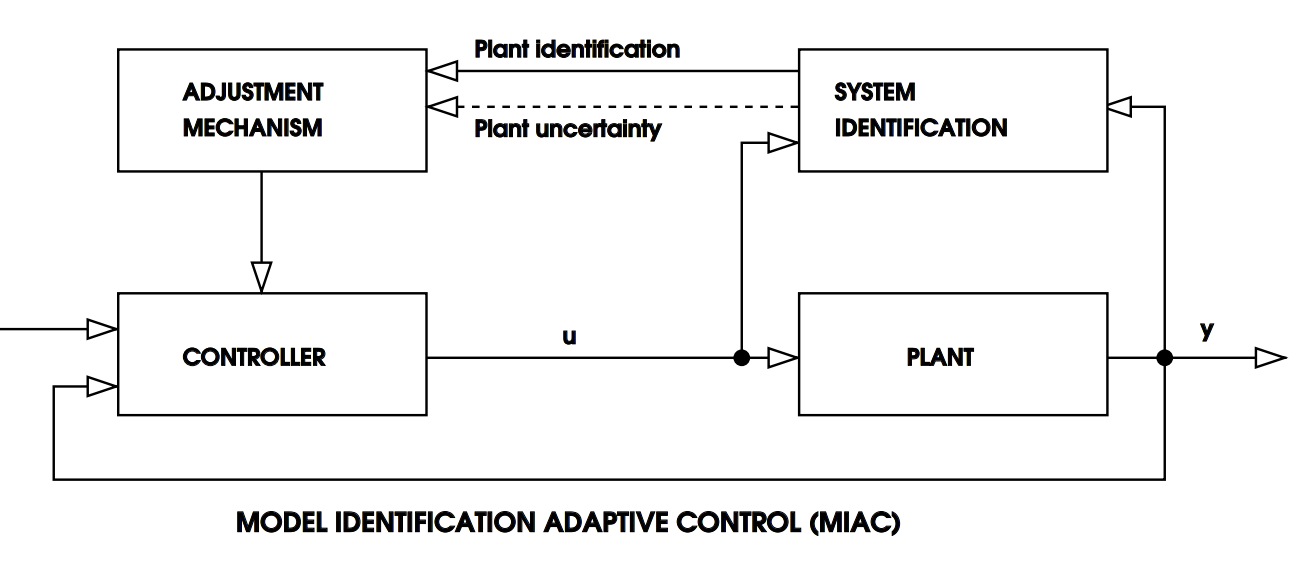
\includegraphics[width = 400pt]{Img/MIAC.png}
	\caption{MIAC blokdiagram}
	\label{fig:MIAC}
\end{figure}

Til system identifikation kan RLS algoritmen bruges. Den fungerer ved løbende at udregne en parameter vektor, som bruges til at opdatere ens controller. Offline RLS vil ikke være det bedste valg til vores bil, da det kræver at man har hele outputtet til at lave estimation på. Det vil sige, at bilen først skal have kørt igennem den rute, man vil have den skal køre.

På \autoref{fig:MIAC} vil RLS algoritmen implementeres i system identifikationsblokken.

\begin{figure}[H]
	\centering
	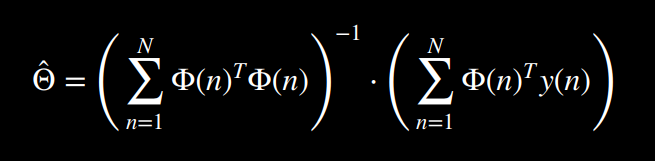
\includegraphics[width = 400pt]{Img/ParameterVektor.png}
	\caption{Parameter vektor}
	\label{fig:ParameterVektor}
\end{figure}
 For at udregne parameter vektoren på \autopageref{fig:ParameterVektor}, skal man have sine målte output data og input data, kaldet phi her.
 
 \begin{figure}[H]
 	\centering
 	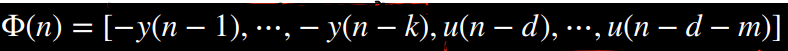
\includegraphics[width = 400pt]{Img/InputOutput.png}
 	\caption{Målte output og input værdier}
 	\label{fig:InputOutput}
 \end{figure}
 Men da det kræver meget computerkræft at invetere matricer omskrives ligningen for thetahat.
 
  \begin{figure}[H]
 	\centering
 	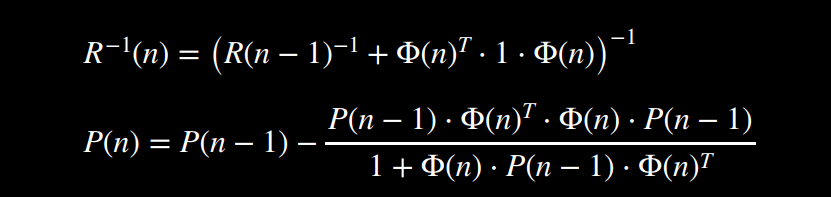
\includegraphics[width = 400pt]{Img/P_rls.png}
 	\caption{Formel for thetahat for RLS online}
 	\label{fig:P_rls}
 \end{figure}
 
 I matlab kan det implementeres på denne måde:
 
 \begin{lstlisting}
 	%Initializering PsiPsi
 	PsiPsi = Psi'*Psi;
 	PsiY = Psi'.*output(1);
 	est_out(1)=0;
 	%Implementation af det digitale filter
 	for n = 2:length(Step)-1
 	
 	Psi_y = [-output(n) Psi_y(1:end-1)];
 	Psi_u = [Step(n-1) Psi_u(1:end-1)];
 	Psi=[Psi_y Psi_u];
 	
 	%Opdater paramter estimation
 	P=P-P*Psi'*Psi*P./(1+Psi*P*Psi');
 	K=P*Psi';
 	Thetahathat=Thetahathat+K*(output(n+1)-Psi*Thetahathat);
 	
 	est_out(n)=Psi*Thetahathat; %Model output y_m(n)
 	end
 \end{lstlisting}